\nTitle{Conception}

%%%%%%%%%%%%%%%%%%%%%%%%%%%%%%%%%%%%%%%%%%%%%%%%%%%%%%%%%%%%
\section{Rappel du contexte}
% Martin


%%%%%%%%%%%%%%%%%%%%%%%%%%%%%%%%%%%%%%%%%%%%%%%%%%%%%%%%%%%%
\section{Choix d'une solution}
\subsection{Présentation des alternatives}

\subsubsection{Points commun des trois solutions}
% Yoann
À l'ouverture d'un fichier, son contenu est copié dans un fichier temporaire --- éventuellement en le structurant de manière adaptée à l'éditeur. Le fichier est indexé de manière à pouvoir accéder aux lignes directement.

Un tampon de taille limitée est créé en mémoire centrale. Lorsque l'utilisateur demande à accéder à des lignes qui n'y sont pas encore chargées, les lignes les plus anciennement accédées sont remplacées par celles qui viennent d'être demandées.

Le tampon est modifié directement au fur et à mesure de la frappe de l'utilisateur, et la ligne modifiée est transférée dans le fichier temporaire dès que l'utilisateur passe à une nouvelle ligne ou demande une sauvegarde du fichier. Le fichier source, quant à lui, est mis à jour sur demande de l'utilisateur (sauvegarde du fichier).

\subsubsection{Solution 1 : structure consécutive}
% Paul
Toute la mémoire est allouée dans des tableaux, d'un seul bloc.

Le fichier temporaire est lui aussi placé dans une structure consécutive dans
un zone contigüe de la mémoire centrale.

La solution est donc homogène : le même mécanisme est mis en place entre la
mémoire centrale et la mémoire secondaire. La compréhension du système est
alors simplifiée.

L'accès est direct : chaque caractère du texte peut être accédé en tant
constant ($O(n)$). De fait, si l'on a besoin uniquement de remplacer des
caractères par d'autres caractères, cette solution est efficace.

De la même manière, si l'on a besoin de rajouter des caractères à la fin du
texte, la solution est là encore très efficace, dans les limites de la mémoire
disponible sur le système.

De plus, cette solution présente l'avantage de ne pas devoir réserver de la
mémoire pour le chaînage, celui-ci n'étant pas présent dans cette solution.
Par contre, nous devons impérativement réserver un \emph{buffer} de taille
importante dès le début, pour éviter la réallocation intempestive. Nous
pourrions envisager d'utiliser la technique bien connue de la réallocation par
pas de $n^2$, c'est à dire réserver la mémoire selon un schéma quadratique, et
donc réserver de plus en plus de mémoire à chaque réallocation.

Par contre, si l'on a besoin d'insérer des caractères au milieu du texte, la
solution est très couteuse. En effet chaque insertion ou suppression de
caractères provoque des opérations en $O(n)$ (où $n$ est le nombre de
caractères entre le point de fin d'insertion ou de suppression et la fin de la
mémoire allouée (le \emph{buffer}). Comme il s'agit d'une opération assez
classique et fréquente, de nombreuses opération sont à prévoir.  Ces opération
sont du type \texttt{memmove()}, qui permet de déplacer des données dans un
\emph{buffer}, et qui a une complexité de $n$.

\subsubsection{Solution 2 : structure mixte}
% Martin

\subsubsection{Solution 3 : structure chaînée}
% Yoann
Toutes les structures de données sont chaînées.

Le ficher temporaire est chaîné grâce à des adresses virtuelles, comme présentées ci-dessous.

\begin{figure}[H]
	\centering
	\caption{Structure d'une adresse virtuelle}
	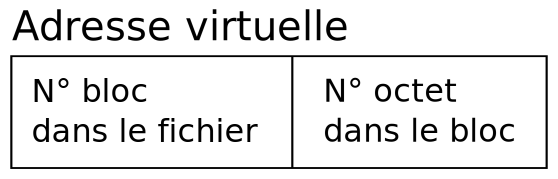
\includegraphics[width=0.5\textwidth]{structure_chainee_temp_adresse_virtuelle}
\end{figure}

Ainsi chaque ligne (y compris la \og ligne 0 \fg virtuelle) fait référence à son successeur et son prédécesseur. On stocke également la longueur de l'information (\og longueur utile \fg) et le nombre d'octets disponibles dans l'enregistrement (\og longueur max \fg, supérieure ou égale à la longueur utile).

\begin{figure}[H]
	\centering
	\caption{Structure du fichier temporaire de la solution 3}
	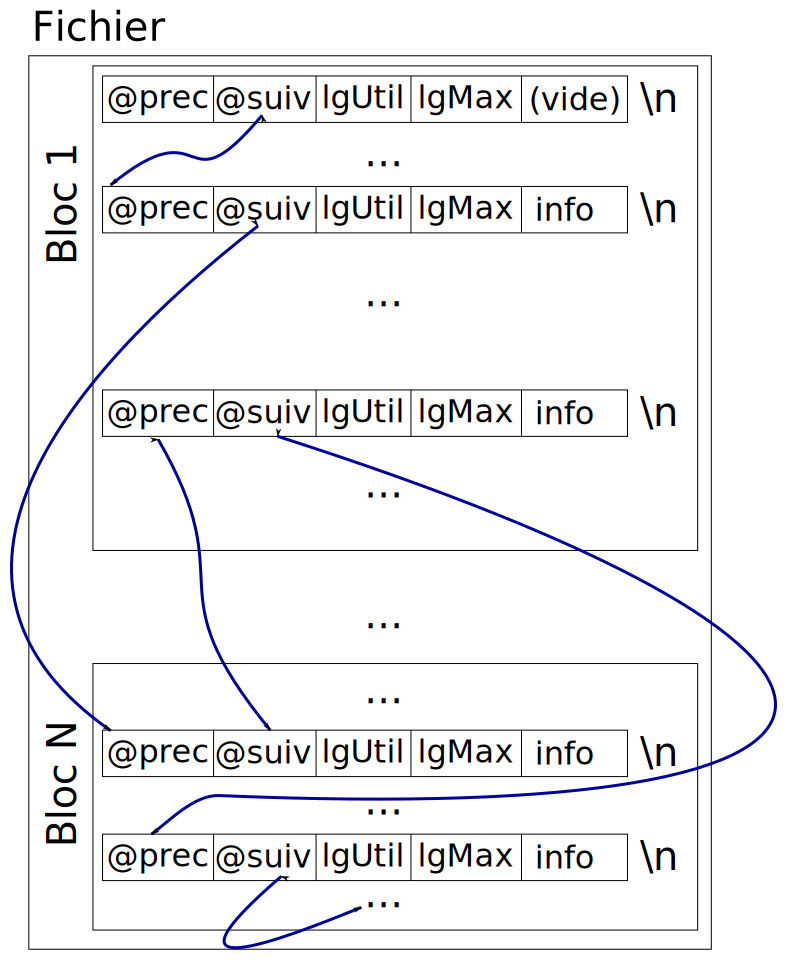
\includegraphics[width=0.6\textwidth]{structure_chainee_temp}
\end{figure}

L'accès direct (lorsque l'utilisateur demande d'accéder à la ligne $l$, par exemple) est possible toutes les $L$ lignes ($L$ à définir) grâce à la table de \textsl{mapping}, qui donne pour chaque bloc la dernière ligne stockée dans celui-ci. Cette table est bien sûr complétée et mise à jour au fur et à mesure de l'édition du fichier (suppressions, ajouts, \ldots). Pour accéder à une ligne non indexée, il suffit d'accéder à une ligne proche et indexée, et de suivre le chaînage (complexité bornée).

Cette table contient bien sûr d'autres informations, comme le montre la représentation suivante.

\newcommand{\TableSolTroisHLine}{\cline{1-5} \cdashline{6-6} \cline{7-7}}
\begin{figure}[H]
	\centering
	\caption{Structure de la table de \textsl{mapping} de la solution 3}
	\vspace{3mm}
	\begin{tabular}{|c|c|c|c|c|c|c|}
		N\textdegree{} ligne & N\textdegree{} bloc & Octet & Chargé & Date dernier accès & (Autres infos) & Adresse MC \\
		\TableSolTroisHLine
		10 & 1 & 156 & Non & 1289135888657534079 & \ldots & \texttt{0x000000}\\
		\TableSolTroisHLine
		\multicolumn{7}{:c:}{} \\
		\multicolumn{7}{:c:}{\ldots} \\
		\multicolumn{7}{:c:}{} \\
		\TableSolTroisHLine
		119 & N & 451 & Oui & 1289135888658945079 & \ldots & \texttt{0x4006d4}\\
		\TableSolTroisHLine
	\end{tabular}
\end{figure}




\subsection{Comparaison des alternatives}
% En commun
% « Mécanisme de justification » : un tableau avec des « + » et des « - » ?

Les critères d'ergonomie et de portabilité ne sont pas pertinents pour la
comparaison des alternatives.
En effet, une bonne ergonomie, au niveau de la conception, sera traduite par une
bonne efficacité, afin d'éviter à l'utilisateur des attentes inutiles.
De plus, nous n'utiliserons pas d'assembleur dans les différentes solutions, se
reposant sur le compilateur C++ pour assurer cette portabilité. Le système sera
donc portable tant que la plateforme dispose d'un compilateur C++.

Nous avons choisis de pondérer ces critères, pour prendre en compte leur
importance respectives.

\begin{table}[H]
	\centering
	\begin{tabular}{l c|c|c|c}
		Critère & Pondération & Solution 1 & Solution 2 & Solution 3 \\
		\hline \hline
		Maintenabilité & 20 & ++ (34) & ++ (35) & +++ (56) \\
		\hline
		Décomposable en couches & 8 & + & ++ & +++ \\
		Homogénéité & 5 & +++ & + & +++ \\
		Couplage entre couches & 5 & + & ++ & +++ \\
		Facilité d'implémentation & 2 & +++ & ++ & + \\
		\hline \hline
		Efficacité & 15 & ++ (27) & ++ (27) & +++ (41) \\
		\hline
		Complexité en insertion & 3 & + & ++ & +++ \\
		Complexité en suppression & 3 & + & ++ & +++ \\
		Complexité au changement de ligne & 3 & + & + & +++ \\
		Complexité de changement de page & 3 & +++ & ++ & +++ \\
		Économie mémoire & 1 & +++ & ++ & + \\
		Complexité de chargement du fichier temporaire & 1 & +++ & ++ & +++ \\
		Complexité de la sauvegarde & 1 & +++ & ++ & + \\
		\hline
		Total & 35 & 61 & 60 & 98 \\
	\end{tabular}
	\vspace{0.5cm}
	\caption{Table comparative des avantages et inconvénients de chaque solution}
\end{table}



%%%%%%%%%%%%%%%%%%%%%%%%%%%%%%%%%%%%%%%%%%%%%%%%%%%%%%%%%%%%
\section{Détail de la solution choisie}

\subsection{...}

\subsection{...}

\subsection{...}

\subsection{...}

\subsection{Proposition d'architecture}
% Découpage modulaire et hiérarchique


%%%%%%%%%%%%%%%%%%%%%%%%%%%%%%%%%%%%%%%%%%%%%%%%%%%%%%%%%%%%
\section{Bilan}
% Bilan de la solution choisie par rapport aux exigeances + réflexions personnelles
